\section{Task 1}
Das folgende Klassendiagramm beschreibt die Struktur unseres Netzwerk Pakets:
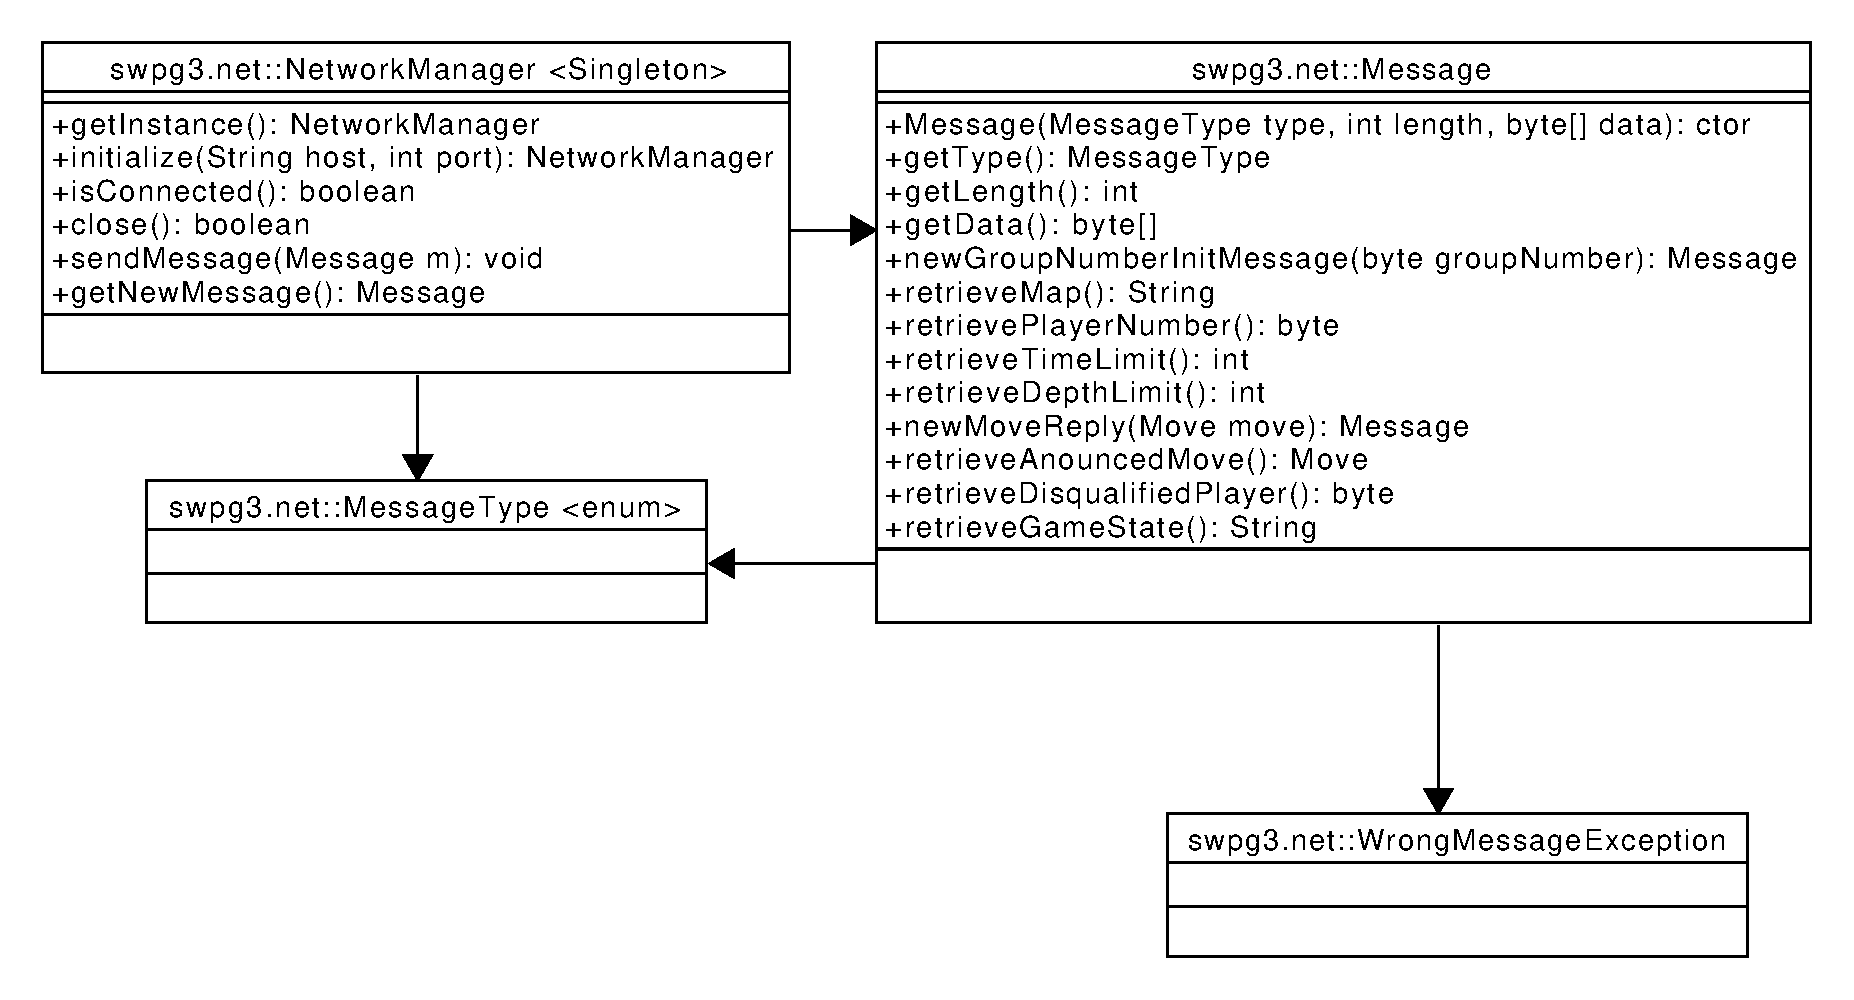
\includegraphics[scale=0.5]{NetPackageClassdiagramm.pdf}

Die Klasse \textit{NetworkManager} regelt dabei das Senden und empfangen von Daten, indem es \textit{Messages} empfängt und sendet.

\textit{Message} ist eine Klasse, die die Nachrichten gemäß Spezifikation repräsentiert. Sie stellt auch Methoden zur Verfügung, um relevante Daten einfach zu extrahieren, bzw. um Nachrichten aus Daten einfach zu erzeugen. Somit ist die Wechselwirkung zum \textit{spwg3.net} gering: Man erbittet den \textit{NetworkManager} um eine Nachricht, und ruft auf der \textit{Message} eine passende Methode auf, um die Daten zu extrahieren. In die andere Richtung ruft man eine statische Methode der \textit{Message}-Klasse auf, um eine Nachricht aus den vorliegenden Daten zu erzeugen, und gibt diese an den \textit{NetworkManager} zum senden.